\chapter{Dynamic Schedule}
The static schedule presented in Chapter~\ref{chap:Static} and commonly throughout the scheduled arrivals literature is fixed for the duration of service. It was intuitively be advantageous to allow the schedule to vary during service. For example, if the service times of the first few customers are longer than expected, then it would be beneficial to schedule the remaining customers to arrive later.

This chapter approaches the problem of choosing a schedule in a similar way to Chapter~\ref{chap:Static}. The aim is to find the arrival time of the first customer and the customer interarrival times that minimise the expected cost. The assumptions on iid service times and punctual customers are the same as Chapter~\ref{chap:Static}.

This dynamic schedule is chosen progressively during service. Immediately after a customer arrives and begins waiting for service, the scheduler chooses the arrival time of the next customer. Most real-world situations are obviously more restrictive than this. It is often not possible to schedule the customer arrivals one-by-one.

Real-world situations would sometimes allow a degree of flexibility in regards to rescheduling customers. The theory is that if the (probably unrealistic) dynamic schedule presented here is significantly better than the static schedule, than the rescheduling ability should be included in real-world models for scheduled arrivals. However, if the dynamic schedule performs similarly to the static schedule than it is likely reasonable to ignore the rescheduling in the model formulation.

\section{Objective Function}
The state $(n, k)$ refers to $n$ customers remaining to be scheduled and $k$ customers currently in the system (i.e., either waiting or being served). The time the next customer is scheduled to arrive relative to the current time is $a$.

The expected cost of a schedule is a linear combination of the expected total customers' waiting time and the total expected server availability time. The expected cost of the current state is a function of the expected cost involved in transitioning to the next state, the expected cost of the next state and the probability of transitioning to the next state (over all possible next states).

For any $n \geq 1$, the probability of transitioning from state $(n, k)$ to state $(n - 1, j)$ over time interval $a$ if the next customer is scheduled to arrive in $a$ time units is denoted by $p_{a} (k, j)$. The expected cost over this transition is denoted by $R_{a} (k, j)$. Note that $j$ is the total number of customers in the system immediately after the next customer's arrival.

For $n \geq 1$, the expected cost of state $(n, k)$ can be computed by the following form of Bellman's equation:
\begin{equation}
	C_{n}^{*} (k) = \min_{a \geq 0} C_{n} (a, k) = \min_{a \geq 0} \left[ \sum_{j = 1}^{k + 1} p_{a} (k, j) \Big( R_{a} (k, j) + C_{n - 1}^{*} (j) \Big) \right]
	\label{Eqn_Bellman}
\end{equation}

Equation~\ref{Eqn_Bellman} is a recursive equation involving $C^{*}$. The optimal dynamic schedule is found by solving for each customer interarrival time $a$ iteratively. The optimal policy $a^{*}$ is the interarrival time that attains the minimum cost whereby
\begin{equation}
	C_{n}^{*} (k) = C_{n} (a^{*}, k) = \min_{a \geq 0} C_{n} (a, k)
\end{equation}

\section{Base Case}
Solving Equation~\ref{Eqn_Bellman} requires a solution for the base case where $n = 0$. The state $(0, k)$ is the state where there are no customers remaining to be scheduled and $k$ customers currently in the system.

Denote the expected waiting time of the customer that is currently in position $i$ as $w_{i}$. This expected waiting time is the summation of the expected service times of all the customers in positions $\{ 1, \ldots, i - 1 \}$. The expected total customers' waiting time for the $k$ remaining customers is the sum of their individual waiting times.
\begin{align}
	\begin{split}
		\mathbb{E} \Big[\text{total customer's waiting time at state $(0, k)$} \Big] & = \sum_{i = 1}^{k} w_{i} = \sum_{i = 1}^{k} \mu (i - 1) \\
		& = \frac{\mu k (k - 1)}{2}
	\end{split}
\end{align}

If there are no customers remaining to be scheduled, then the expected total server availability time is the expected time until the customer currently in the last position in the queue finishes service. This time is the summation of the expected service times of all the customers currently in the system.
\begin{equation}
	\mathbb{E} \Big[\text{total server availability time at state $(0, k)$} \Big] = \sum_{i = 1}^{k} \mu = k \mu
\end{equation}

The per unit costs $c_{W}$ and $c_{S}$ are defined as before in Chapter~\ref{chap:Static}. The cost of the base case is thus given by
\begin{equation}
 	C_{0}^{*} (k) = c_{W} \frac{\mu k (k - 1)}{2} + c_{S} k \mu
\end{equation}

In order to compare $C_{0}^{*} (k)$ with the cost of the static schedule, need to scale it by dividing by $(c_{S} + c_{W})$ and defining $\gamma = \frac{c_{S}}{c_{S} + c_{W}}$.
\begin{equation}
	C_{0}^{*} (k) = (1 - \gamma) \frac{\mu k (k - 1)}{2} + \gamma k \mu
\end{equation}

\section{Erlang Distribution}
The transition probability and expected transition cost for the dynamic schedule depend on the cdf and conditional expectation of the Erlang distribution, which are shown here.

Denote the service time of the customer that is currently in position $i$ in the queue as $S_{i}$. For $n$ customers, the service times $S_{1}, \ldots, S_{n}$ are iid exponential random variables with mean $\mu$.

For $r \geq 1$, the waiting time of the customer in position $(r + 1)$ is given by
\begin{equation}
	X = \sum_{i = 1}^{r} S_{i} \sim \text{Erlang}(r, \mu)
\end{equation}

which has the pdf
\begin{equation}
	f (x; r) = \frac{1}{\mu (r - 1)!} \left( \frac{x}{\mu} \right)^{r - 1} \mathrm{e}^{\frac{-x}{\mu}}
\end{equation}

The cdf of the Erlang distribution is
\begin{equation}
	F (a; r) = \mathbb{P} (X \leq a) = \begin{cases} 0 & \text{for $a = 0$} \\ 1 - \sum_{i = 0}^{r - 1} \frac{1}{i!} \left( \frac{a}{\mu} \right)^{i} \mathrm{e}^{\frac{-a}{\mu}} & \text{for $a > 0$} \end{cases}
\end{equation}

For $r \geq 1$, $F (a; r)$ is continuous for $a \geq 0$ as
\begin{equation}
	\lim_{a \to 0^{+}} F (a; r) = 0 = F (0; r)
\end{equation}

The conditional expectation of the Erlang distribution can be shown to be
\begin{equation}
	G (a; r) = \mathbb{E} [X | X \leq a] = \begin{cases} 0 & \text{for $a = 0$} \\ (\mu r) \frac{F (a; r + 1)}{F (a; r)} & \text{for $a > 0$} \end{cases}
\end{equation}

This expression makes intutive sense. For $a > 0$ and $r \geq 1$, $\frac{F (a; r + 1)}{F (a; r)} < 1$. In addition, the mean of the Erlang distribution is $\mathbb{E} [X] = \mu r$. Thus, for $a > 0$ and $r \geq 1$, $\mathbb{E} [X | X \leq a] < \mathbb{E} [X]$ as expected.

Moreover, 
\begin{equation}
	\lim_{a \to \infty} \frac{F (a; r + 1)}{F (a; r)} = \frac{\displaystyle \lim_{a \to \infty} F (a; r + 1)}{\displaystyle \lim_{a \to \infty} F (a; r)} = \frac{1}{1} = 1
\end{equation}

Thus, $\displaystyle \lim_{a \to \infty} \mathbb{E} [X | X \leq a] = \mathbb{E} [X]$ as expected.

\section{Transition Probability}
The transition probability $p_{a} (k, j)$ is the probability that the queue length changes from $k$ customers initially to $j$ customers on the arrival of the next customer after $a$ time units. In other words, it is the probability that there are $k - (j - 1)$ departures from the queue over a time interval of length $a$.

 Can compute the transition probability on a case by case basis. The full derivation is included in the appendix and only the final equation is presented here.
\begin{equation}
	p_{a} (k, j) = \begin{cases}
		\mathbbm{1} (j = 1) & \text{for $k = 0$} \\
		F (a; k) & \text{for $k \geq 1, j = 1$} \\
		F (a; k - j + 1) - F (a; k - j + 2) & \text{for $k \geq 1, 2 \leq j \leq k$} \\
		1 - F (a; 1) & \text{for $k \geq 1, j = (k + 1)$} \\
		0 & \text{otherwise}
	\end{cases}
\end{equation}

\section{Expected Transition Cost}
The expected transition cost is the expected cost of transitioning from state $(n, k)$ to state $(n - 1, j)$ where the next customer is scheduled to arrive in $a$ time units.

In a similar way to the transition probability, the expected transition cost is derived on a case by case basis. To compare the dynamic schedule with the static schedule, the cost is scaled by dividing by $(c_{S} + c_{W})$ and defining $\gamma = \frac{c_{S}}{c_{S} + c_{W}}$. The full derivation is included in the appendix and the final equation is presented here.
\begin{multline}
	R_{a} (k, j) \\
	= \begin{cases}
		\gamma a & \text{for $k \in \{ 0, 1 \}$} \\
		(1 - \gamma) \frac{G (a; k) (k - 1)}{2} + \gamma a & \text{for $k \geq 2, j = 1$} \\
		(1 - \gamma) \left[ a (j - 2) + \frac{G (a; k - (j - 1)) [k - (j - 2)]}{2} \right] + \gamma a & \text{for $k \geq 2, 2 \leq j \leq k$} \\
		(1 - \gamma) \big[ a (j - 2) \big] + \gamma a & \text{for $k \geq 2, j = (k + 1)$}
	\end{cases}
\end{multline}

\section{Example Models}
\subsection{State (3, 2)}
Assume that the mean service time $\mu = 1$. In addition, assume that the per unit time costs of the customers' waiting time ($c_{W}$) and server's total availability time ($c_{S}$) are both equal such that $\gamma = 0.5$. Under these assumptions, the expected cost of the state $(3, 2)$ for various values of $a$ is given by the following expression, which is continuous for $a \geq 0$.
\begin{equation*}
	C_{3} (a, 2) =
	\begin{cases}
 		4.94 & \text{where $a = 0$} \\
 		2.76 + \frac{a}{2} + \exp (- a) \left( \frac{a^{2}}{4} + 1.65 a + 2.18 \right) - \frac{a^{2}}{2 [\exp (a) - 1]} & \text{where $a > 0$}
	\end{cases}
\end{equation*}

\begin{figure}[htb]
	\centering
	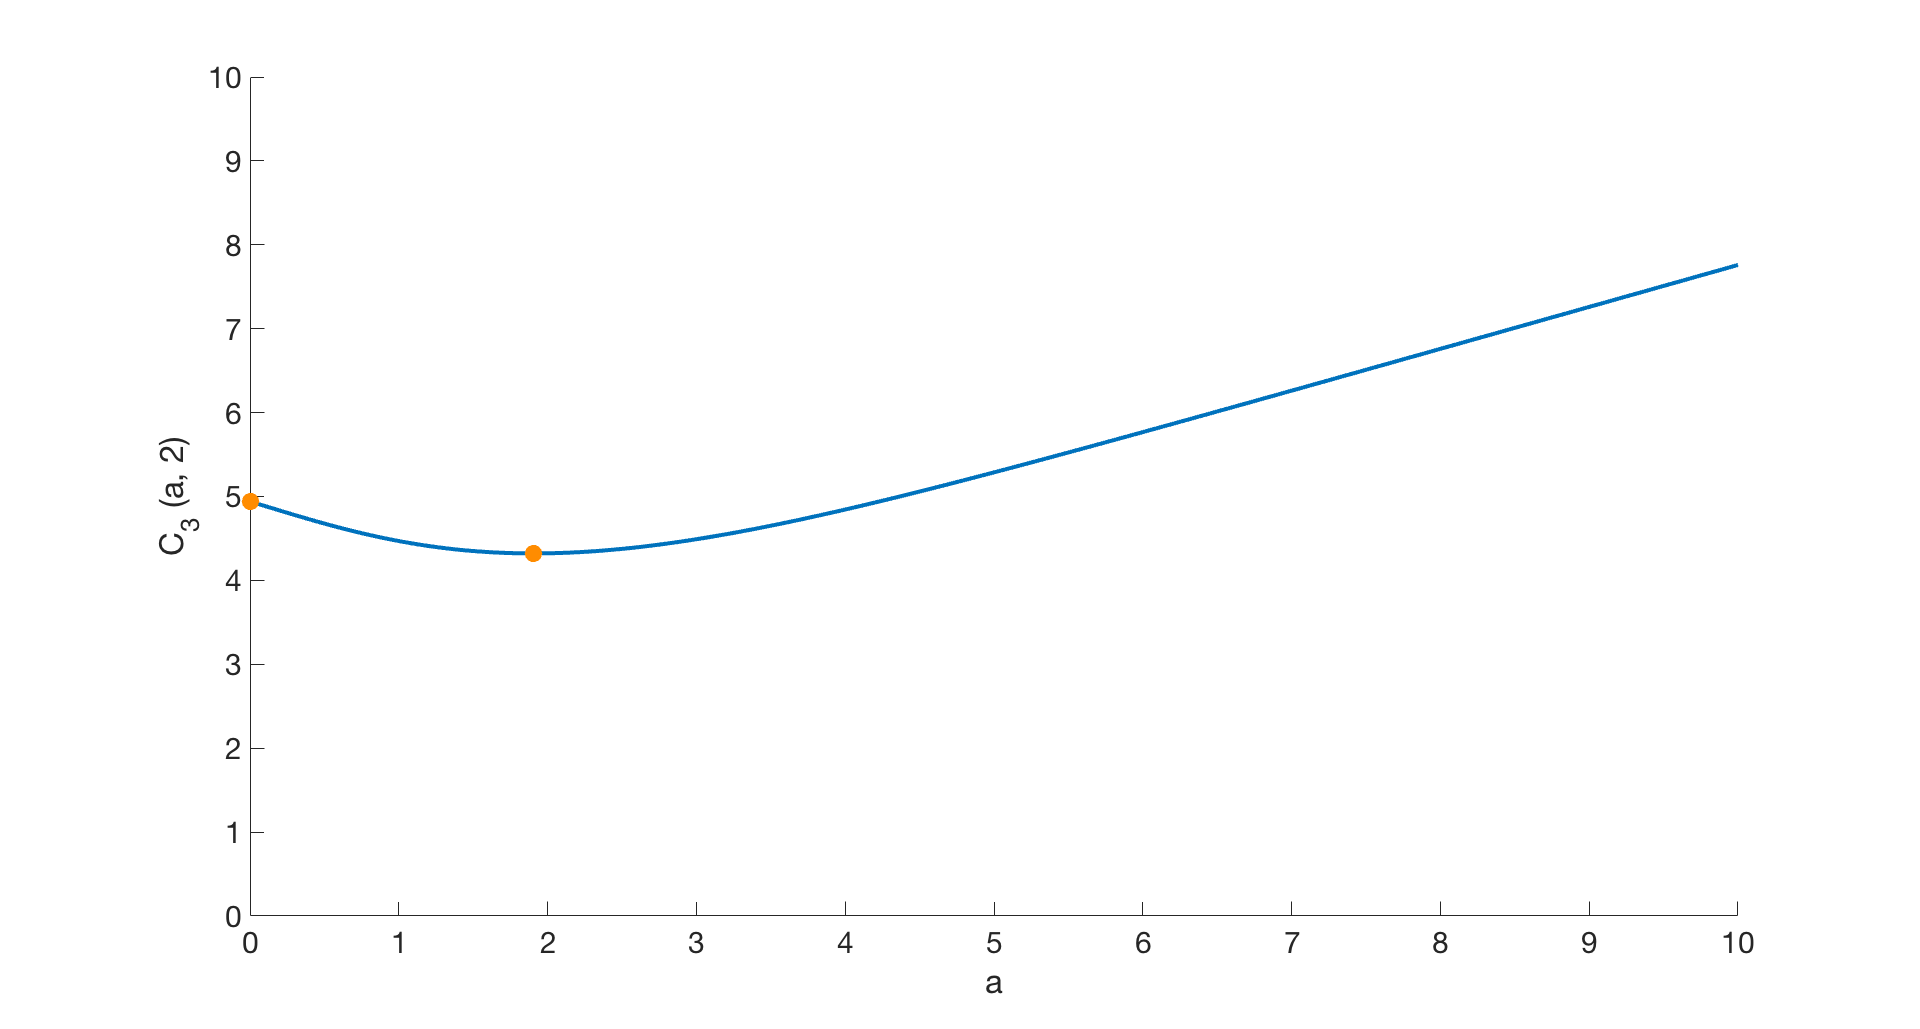
\includegraphics[width = 0.85\textwidth]{Graph_3_2.png}
	\caption{Cost of state with $n = 3$ and $k = 2$ for $a \in [0, 10]$ where $\mu = 1$ and $\gamma = 0.5$.}
	\label{Graph_3_2}
\end{figure}
Figure~\ref{Graph_3_2} plots this cost for $a \in [0, 10]$ to visualise the relationship between the cost and $a$. The only value of $a$ where $\frac{\partial}{\partial a} C_{3} (a, 2) = 0$ is $1.90$. Thus, the set of possible policies $\mathcal{A}$ is $\{ 0, 1.90 \}$ whereby there are two possible policies labelled as orange dots on Figure~\ref{Graph_3_2}. Moreover, note that as $a$ increases beyond 2, the cost increases approximately linearly.

The optimal policy $a^{*}$ that minimises $C_{3} (a, 2)$ is $1.90$ where the cost is $8.64$. If (on arrival of a customer) there are two customers in the system and three customers remaining to be scheduled, then the next customer should be scheduled to arrive in $1.90$ time units. This is slightly below the expected service time of the two customers in the system to account for the availability cost of the server.

\subsection{Model for Six Customers}
Assume there are six customers that need to be scheduled for service who all have a mean service time $\mu = 1$. The initial state is $(6, 0)$, and the possible states during service are all states in the set
\begin{equation}
	\Big\{ (n, k) \in \{ 0, 1, \ldots, 6 \}^{2} : n + k \leq 6 \Big\}
\end{equation}

\begin{table}[htb]
	\centering
	\begin{tabular}{c c c || c | c | c | c | c | c | c}
		& & & \multicolumn{7}{c}{Current Number in System ($k$)} \\
		& & & 0 & 1 & 2 & 3 & 4 & 5 & 6 \\ \hline \hline
		\parbox[t]{2mm}{\multirow{7}{*}{\rotatebox[origin=c]{90}{Customers to be}}} & \parbox[t]{2mm}{\multirow{7}{*}{\rotatebox[origin=c]{90}{Scheduled ($n$)}}} & 0 & 0 & 0.5 & 1.5 & 3 & 5 & 7.5 & 10.5 \\
		& & 1 & 0.5 & 1.35 & 2.49 & 4.02 & 5.98 & 8.37 \\
		& & 2 & 1.35 & 2.26 & 3.41 & 4.94 & 6.89 & \\
		& & 3 & 2.26 & 3.18 & 4.32 & 5.86 & & \\
		& & 4 & 3.18 & 4.09 & 5.24 & & & \\
		& & 5 & 4.09 & 5.01 & & & & \\
		& & 6 & 5.01 & & & & &
	\end{tabular}
	\caption{Cost of possible states for 6 total customers}
	\label{Cost_6_Customers}
\end{table}

Table~\ref{Cost_6_Customers} displays the calculated expected costs for each possible state if there are six total customers (assuming $\gamma = 1$). The cost of the initial state is $5.01$, thus the expected cost of servicing six customers with a dynamic schedule is $5.01$.

Note for $n \geq 1$, $C_{n}^{*} (0) = C_{n - 1}^{*} (1)$. This is due to the fact that if there are no customers currently in the system (e.g., initially), then it is always optimal to schedule the next arrival immediately. The expected cost thus doesn't change as the next arrival occurs immediately.

The worst state on Table~\ref{Cost_6_Customers} is the state $(0, 6)$, which is all six customers in the system. This can occur if all six customers are scheduled to arrive immediately (to ensure minimal server availability time) or if the first customer has an extremely long service time.

\begin{table}[htb]
	\centering
	\begin{tabular}{c c c || c | c | c | c | c | c}
		& & & \multicolumn{6}{c}{Current Number in System ($k$)} \\
		& & & 0 & 1 & 2 & 3 & 4 & 5 \\ \hline \hline
		\parbox[t]{2mm}{\multirow{6}{*}{\rotatebox[origin=c]{90}{Customers to be}}} & \parbox[t]{2mm}{\multirow{6}{*}{\rotatebox[origin=c]{90}{Scheduled ($n$)}}} & 1 & 0 & 0.69 & 1.76 & 2.83 & 3.86 & 4.85 \\
		& & 2 & 0 & 0.83 & 1.90 & 2.95 & 3.96 \\
		& & 3 & 0 & 0.83 & 1.90 & 2.95 & \\
		& & 4 & 0 & 0.83 & 1.90 & & \\
		& & 5 & 0 & 0.83 & & & \\
		& & 6 & 0 & & & &
	\end{tabular}
	\caption{Optimal policy for each possible states for 6 total customers}
	\label{Policy_6_Customers}
\end{table}

Table~\ref{Policy_6_Customers} displays the corresponding arrival times for the costs in Table~\ref{Cost_6_Customers}. This table does not include any optimal times for $n = 0$, as there is no next customer to schedule in those states.

The first pattern to notice is (as discussed earlier) if there are no customers currently waiting (i.e., $k = 0$), then the optimal policy is to schedule the next arrival immediately. This makes intutive sense as scheduling the next arrival immediately minimises the total server availability time without affecting the total customers' waiting times.

As $k$ increases for fixed $n$, the optimal scheduled arrival time $a^{*}$ appears to increase at a decreasing rate. The optimal $a^{*}$ increases by approximately $\mu$ for each extra $k$.

In contrast, for $n \geq 2$, $a^{*}$ appears to be constant at a value slightly less than $\mu k$ (i.e., the expected time for the system to be empty). This is due to the server availability cost leading to a desire for the next customer to arrive just before the queue becomes empty.


































